\documentclass{scrartcl}

\usepackage[ngerman]{babel}
\usepackage[utf8]{inputenc}
\usepackage[T1]{fontenc}
\usepackage{graphicx}
\usepackage{amsmath}
\usepackage{chemmacros}
\usepackage{color}
\usepackage{enumitem}
\usepackage{icomma}
\usepackage{titlesec}
\usepackage{tikz}
\usepackage{adjustbox}
\usepackage{geometry}
 \geometry{
 a4paper,
 total={170mm,250mm},
 left=20mm,
 top=20mm,
 }

\usepackage[activate={true,nocompatibility},final]{microtype} % better font-rendering
\usepackage[bitstream-charter]{mathdesign} % bitstream font
\titleformat{\section}[hang]{
	\usefont{T1}{bch}{b}{n}\selectfont} % "bch" - Bitstream Character, "b" - bold 
	{} % label
	{0em} % horizontal separation between label and title body
	{\hspace{-0.4pt}\Large \thesection\hspace{0.6em}} % code preceding the title
	[] % additional code following the title body
\titleformat{\subsection}[hang]{
	\usefont{T1}{bch}{b}{n}\selectfont}
	{}
	{0em}
	{\hspace{-0.4pt}\large \thesubsection\hspace{0.6em}}
	[]
\titleformat{\subsubsection}[hang]{
	\usefont{T1}{bch}{b}{n}\selectfont}
	{}
	{0em}
	{\hspace{-0.4pt}\thesubsubsection\hspace{0.6em}}
	[]


\chemsetup{ modules = all }
%\usepackage[version=4]{mhchem}
\chemsetup[redox]{pos=top} % oxid. numbers on top
\usepackage{chemfig}

\newlength{\drop}
\usepackage{float}

\begin{document}
  \begin{titlepage}
    \drop=0.1\textheight
    \centering
    \vspace*{\baselineskip}
    \rule{\textwidth}{1.6pt}\vspace*{-\baselineskip}\vspace*{2pt}
    \rule{\textwidth}{0.4pt}\\[\baselineskip]
    {\LARGE Versuch 1-1 (ABS)\\[0.3\baselineskip] Optische Absorptionsspektroskopie}\\[0.2\baselineskip]
    \rule{\textwidth}{0.4pt}\vspace*{-\baselineskip}\vspace{3.2pt}
    \rule{\textwidth}{1.6pt}\\[\baselineskip]
    \scshape
    {Praktische Einführung in die Chemie\par}
    \vspace*{2\baselineskip}
    \vfill
    {\scshape Versuchtstag:} \        {\large 17.05.2017}\par
  \end{titlepage}
\section{Theorieteil}
\subsection{Grundlagen}
Die Absorptionsspektroskopie beruht im Wesentlichen auf der Analyse der Veränderung, die - typischer Weise \emph{monochromatisches} - Licht beim Durchgang durch eine Probe erfährt. Dazu wird eben solch monochromatisches Licht bestimmter Wellenlänge $\lambda$ durch eine Probe der Konzentration $c_0$ mit der Dicke $d$ geschickt. Nach dem \emph{Lambert-Beer’schen} Gesetz gilt folgende Beziehung der Ursprünglichen Intensität $I_0$ des emmitierten Lichts und der des nach dem Durchscheinen der Probe detektierten Lichts $I_1$:
\begin{equation}\label{eq:LamBeer}
	I_1(\lambda) = I_0(\lambda)\cdot e^{-\epsilon(\lambda)\cdot c_0\cdot d}
\end{equation}
Wobei $\epsilon(\lambda)$ der sogenannte stoffabhängige molare Extinktionskoeffizient, der das spezifische Absorptionvermögen eines Stoffes beschreibt, ist. 

Bei der Absorption wird die Energie des Lichtes auf das Molekül übertragen. Abhängig von dem Betrag der Energie, also der Wellenlänge des Lichts hat dies unterschiedliche Auswirkungen. Im folgenden wird die Anregung eines Elektrons des Moleküls betrachtet. Zwecks Vereinfachung wird das Elektron in einem Kasten gewisser Länge $a$ gedacht. Aus der Schrödingergleichung lässt sich dem Teilchen folgende Energie zuordnen: 
\begin{equation}
	E_n = \frac{n^2\cdot h^2}{8\cdot m\cdot a^2}
\end{equation}
Wobei $m$ die Masse, $n \in \mathbb{N}$ die Quantenzahl des Elektrons und $h$ das Plancksche Wirkungsquantum ist. Eine höhere Quantenzahl steht für einen energetisch höheren, sprich angeregten Zustand. Die Energie, die aufgebracht werden muss, um das Teilchen von einem Grundzustand $n_G$ in einen angeregten $n_A$ zu versetzen, ist die Differenz der zugehörigen Energieniveaus: $\Delta E=E_A - E_G$. Entspricht die Energie des einfallenden Lichts $E = h\cdot f$ ($f$ ist die Frequenz des Lichts) diesem $\Delta E$ wird das Elektron angeregt. 
Denkt man sich nun $N$ Elektronen in einem ebensolchen Kasten, kommt das Pauliprinzip zu tragen, das besagt, dass Elektronen, die sich in ihren Quantenzahlen gleichen nicht das selbe Energieniveau besetzten dürfen, folglich also maximal zwei Elektronen mit entgegengeseztem Spin sich auf dem gleichen Niveau befinden können. Daraus folgt, dass für $N$ Elektronen $\frac{N}{2}$ Energieniveaus existieren. Eine Anregung eines Elektrons kann nur vom höchsten besetzten Niveau in das niedrigste Unbesetzte erfolgen, also 
\begin{subequations}
	\begin{align}
\Delta E&=\frac{h^2}{8\cdot m\cdot a^2}\cdot(N+1)\\
E &= h\cdot f = h\cdot \frac{c}{\lambda}
\end{align}
\end{subequations}
was wie zuvor mit der Energie des absorbierten Licht , mit $c$ als der Lichtgeschwindigkeit, übereinstimmt.
Diese Überlegung ist bezüglich der Realität stark vereinfacht, jedoch können beispielsweise manche organische Verbindung als solche Kasten gedacht werden, in dem sich die $\pi$-Elektronen der Bindungen befinden. 
\subsection{Bestimmung der Dissoziationskonstante}
Mit Hilfe der Absorptionsspektroskopie lässt sich die Dissoziationskonstante eines Säure bestimmen. Hierzu sind einige grundlegende Dinge zur Verständnis wichtig.

Eine Säure \ch{HA} dissoziiert folgendermaßen:
\begin{subequations}
	\begin{align}
		\text{HA} &\rightleftharpoons \text{A}^- + \text{H}^+ \\
		K_S &= \frac{[\text{H}^+] \cdot [\text{A}^-]}{[\text{HA}]} \label{eq:Ks}
	\end{align}
\end{subequations}
Die Gleichgewichtskonstante dieser Reaktion wird auch als Dissoziationskonstante der Säure bezeichnet. Weiterhin gilt, dass die Summe der Konzentration der bereits dissoziierten Säure und der der nicht disoziierten gleich der Ausgangskonzentration $c_0$ sein müssen: \ch{[HA] + [A^-] = c_0}

Aus Gleichung \ref{eq:LamBeer} folgt: 
\begin{equation}\label{eq:Extk}
	E(\lambda)_{\text{A}^-}=\ln{\frac{I_0(\lambda)}{I_1(\lambda)}} = \epsilon(\lambda)_{\text{A}^-}\cdot c_0\cdot d
\end{equation}
Hieraus lässt sich durch Messungen $\epsilon(\lambda)$ bestimmten.

\section{Versuche}
\subsection{Bestimmung der Länge eines eindimensionalen Potentialtopfs}
\subsubsection{Aufgabenstellung}
Messung des Absorptionsspektrums einer $\beta$ -Carotinlösung und Bestimmung der Länge eines Potentialtopfs.
\subsubsection{Versuchsdurchführung}
Zu erst wurde das Spektrometer kalibriert in dem beide Küvetten mit dem Lösungsmittel(Cyclohexan) auf ca. 2 cm befüllt wurden und dann in den Spektrometer gestellt wurden. Danach wurde die vordere Küvette ausgetauscht und mit der $\beta$ -Carotinlösung befüllt. Dann wurde die Lösung im Bereich von 500 - 330 nm vermessen und das entstandene Diagramm ausgedruckt und per Computer das Maxima bestimmt.
\begin{figure}[h]
	\centering
	\caption{Messwerte zu Versuch 1}
	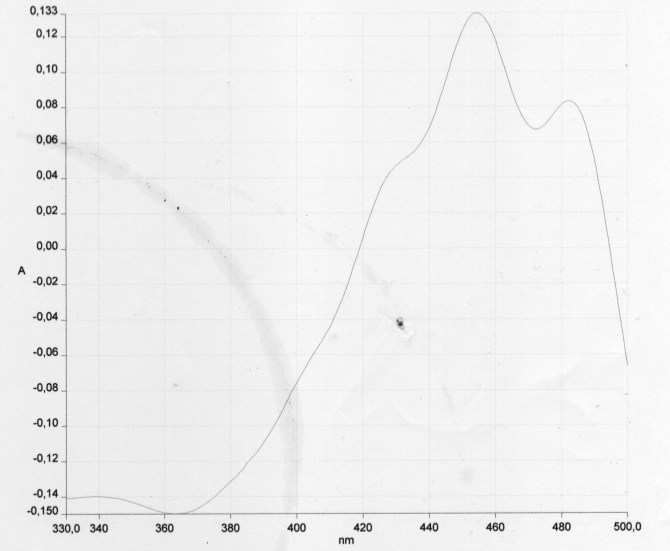
\includegraphics[scale=.5]{Kurve1.png}
\end{figure}
\subsubsection{Auswertung}
Das gemessene Absorptionsmaximum $E_{\lambda,\text{max}}$ liegt im Versuch bei  $\lambda$ = 454,3 nm. Die Energie des Lichts beträgt dann nach:
\begin{equation*}
\Delta E = \frac{h\cdot c}{\lambda \textsubscript{max}} = 4,37\cdot 10\textsuperscript{-19}J.
\end{equation*}
Dabei wurde mit $c= 2,998\cdot 10^8 \frac{m}{s}$ und mit $h = 6,626\cdot 10\textsuperscript{-34}$ Js gerechnet. Diese Energie kann gleichgesetzt werden mit
\begin{equation*}
\Delta E = \frac{h\textsuperscript{2} (N+1)}{8 m a\textsuperscript{2}}.
\end{equation*}
\newpage
Formt man diese Gleichung nach a um:

\begin{equation}
	a = \sqrt{\frac{h^2 (N+1)}{8m \Delta E}} = \sqrt{\frac{6,626\cdot10^{-34}\cdot(22+1)}{8\cdot9,109\cdot10^{-31}}} = 1,78 \text{ nm}
\end{equation}
und setzt die Werte ein, hier N = Anzahl der Elektronen (hier 22), $m = 9,109\cdot 10\textsuperscript{-31}$ kg (Masse eines Elektrons) und $h = 6,626\cdot 10\textsuperscript{-34}$ Js, so ergibt sich ein Wert für a mit $a= 1,78 \text{ nm}$.
Der elektronische Übergang kann mit Hilfe des Pauliprinzip festgestellt werden. Das $\beta$ -Carotin besitzt im Delokalisationsbereich N=22 Elektronen. Somit gilt:
\begin{align*}
n\textsubscript{g} &= \frac{N}{2} = 11 \\
n\textsubscript{a} &= \frac{N}{2} +1 = 12 \\
\end{align*}
Dies entspricht einem elektronischen Übergang vom Grundzustand n\textsubscript{g} = 11 in den angeregten Zustand n\textsubscript{a} = 12. Der theoretische Wert für a kann mit Hilfe trigonometrischer Eigenschaften ermittelt werden, mit der mittleren Bindungslänge s = 139,8 pm und dem Bindungswinkel $\phi$ = 120 = $\frac{\pi}{6}$. Mit 22 $\pi$-Elektronen besitzt die Kette 21 Bindungen, wodurch sich ein a mit:
\begin{equation*}
	a = 21 \cdot \cos(\frac{\pi}{6}) \cdot s = 2,542 \text{nm}
\end{equation*}
ergibt. Vergleicht man nun den gemessenen Wert mit dem errechneten ergibt sich eine Abweichung von ca. 29,98\%.
	\begin{figure}[H]
	\centering
	\caption{Messwerte zu Versuch 2}
	% GNUPLOT: LaTeX picture
\setlength{\unitlength}{0.240900pt}
\ifx\plotpoint\undefined\newsavebox{\plotpoint}\fi
\sbox{\plotpoint}{\rule[-0.200pt]{0.400pt}{0.400pt}}%
\begin{picture}(1500,900)(0,0)
\sbox{\plotpoint}{\rule[-0.200pt]{0.400pt}{0.400pt}}%
\put(191.0,131.0){\rule[-0.200pt]{4.818pt}{0.400pt}}
\put(171,131){\makebox(0,0)[r]{$-7$}}
\put(1419.0,131.0){\rule[-0.200pt]{4.818pt}{0.400pt}}
\put(191.0,222.0){\rule[-0.200pt]{4.818pt}{0.400pt}}
\put(171,222){\makebox(0,0)[r]{$-6.8$}}
\put(1419.0,222.0){\rule[-0.200pt]{4.818pt}{0.400pt}}
\put(191.0,313.0){\rule[-0.200pt]{4.818pt}{0.400pt}}
\put(171,313){\makebox(0,0)[r]{$-6.6$}}
\put(1419.0,313.0){\rule[-0.200pt]{4.818pt}{0.400pt}}
\put(191.0,404.0){\rule[-0.200pt]{4.818pt}{0.400pt}}
\put(171,404){\makebox(0,0)[r]{$-6.4$}}
\put(1419.0,404.0){\rule[-0.200pt]{4.818pt}{0.400pt}}
\put(191.0,495.0){\rule[-0.200pt]{4.818pt}{0.400pt}}
\put(171,495){\makebox(0,0)[r]{$-6.2$}}
\put(1419.0,495.0){\rule[-0.200pt]{4.818pt}{0.400pt}}
\put(191.0,586.0){\rule[-0.200pt]{4.818pt}{0.400pt}}
\put(171,586){\makebox(0,0)[r]{$-6$}}
\put(1419.0,586.0){\rule[-0.200pt]{4.818pt}{0.400pt}}
\put(191.0,677.0){\rule[-0.200pt]{4.818pt}{0.400pt}}
\put(171,677){\makebox(0,0)[r]{$-5.8$}}
\put(1419.0,677.0){\rule[-0.200pt]{4.818pt}{0.400pt}}
\put(191.0,768.0){\rule[-0.200pt]{4.818pt}{0.400pt}}
\put(171,768){\makebox(0,0)[r]{$-5.6$}}
\put(1419.0,768.0){\rule[-0.200pt]{4.818pt}{0.400pt}}
\put(191.0,859.0){\rule[-0.200pt]{4.818pt}{0.400pt}}
\put(171,859){\makebox(0,0)[r]{$-5.4$}}
\put(1419.0,859.0){\rule[-0.200pt]{4.818pt}{0.400pt}}
\put(191.0,131.0){\rule[-0.200pt]{0.400pt}{4.818pt}}
\put(191,90){\makebox(0,0){$0.001$}}
\put(191.0,839.0){\rule[-0.200pt]{0.400pt}{4.818pt}}
\put(399.0,131.0){\rule[-0.200pt]{0.400pt}{4.818pt}}
\put(399,90){\makebox(0,0){$0.00105$}}
\put(399.0,839.0){\rule[-0.200pt]{0.400pt}{4.818pt}}
\put(607.0,131.0){\rule[-0.200pt]{0.400pt}{4.818pt}}
\put(607,90){\makebox(0,0){$0.0011$}}
\put(607.0,839.0){\rule[-0.200pt]{0.400pt}{4.818pt}}
\put(815.0,131.0){\rule[-0.200pt]{0.400pt}{4.818pt}}
\put(815,90){\makebox(0,0){$0.00115$}}
\put(815.0,839.0){\rule[-0.200pt]{0.400pt}{4.818pt}}
\put(1023.0,131.0){\rule[-0.200pt]{0.400pt}{4.818pt}}
\put(1023,90){\makebox(0,0){$0.0012$}}
\put(1023.0,839.0){\rule[-0.200pt]{0.400pt}{4.818pt}}
\put(1231.0,131.0){\rule[-0.200pt]{0.400pt}{4.818pt}}
\put(1231,90){\makebox(0,0){$0.00125$}}
\put(1231.0,839.0){\rule[-0.200pt]{0.400pt}{4.818pt}}
\put(1439.0,131.0){\rule[-0.200pt]{0.400pt}{4.818pt}}
\put(1439,90){\makebox(0,0){$0.0013$}}
\put(1439.0,839.0){\rule[-0.200pt]{0.400pt}{4.818pt}}
\put(191.0,131.0){\rule[-0.200pt]{0.400pt}{175.375pt}}
\put(191.0,131.0){\rule[-0.200pt]{300.643pt}{0.400pt}}
\put(1439.0,131.0){\rule[-0.200pt]{0.400pt}{175.375pt}}
\put(191.0,859.0){\rule[-0.200pt]{300.643pt}{0.400pt}}
\put(30,495){\makebox(0,0){ln K}}
\put(815,29){\makebox(0,0){1/T}}
\put(1279,818){\makebox(0,0)[r]{K gemittelt}}
\put(1412,771){\makebox(0,0){$+$}}
\put(965,605){\makebox(0,0){$+$}}
\put(587,362){\makebox(0,0){$+$}}
\put(306,138){\makebox(0,0){$+$}}
\put(1349,818){\makebox(0,0){$+$}}
\put(1279,777){\makebox(0,0)[r]{y = 5219.6804*x -12.2624}}
\put(1299.0,777.0){\rule[-0.200pt]{24.090pt}{0.400pt}}
\put(306,177){\usebox{\plotpoint}}
\multiput(306.00,177.59)(0.943,0.482){9}{\rule{0.833pt}{0.116pt}}
\multiput(306.00,176.17)(9.270,6.000){2}{\rule{0.417pt}{0.400pt}}
\multiput(317.00,183.59)(0.798,0.485){11}{\rule{0.729pt}{0.117pt}}
\multiput(317.00,182.17)(9.488,7.000){2}{\rule{0.364pt}{0.400pt}}
\multiput(328.00,190.59)(0.943,0.482){9}{\rule{0.833pt}{0.116pt}}
\multiput(328.00,189.17)(9.270,6.000){2}{\rule{0.417pt}{0.400pt}}
\multiput(339.00,196.59)(0.798,0.485){11}{\rule{0.729pt}{0.117pt}}
\multiput(339.00,195.17)(9.488,7.000){2}{\rule{0.364pt}{0.400pt}}
\multiput(350.00,203.59)(1.033,0.482){9}{\rule{0.900pt}{0.116pt}}
\multiput(350.00,202.17)(10.132,6.000){2}{\rule{0.450pt}{0.400pt}}
\multiput(362.00,209.59)(0.943,0.482){9}{\rule{0.833pt}{0.116pt}}
\multiput(362.00,208.17)(9.270,6.000){2}{\rule{0.417pt}{0.400pt}}
\multiput(373.00,215.59)(0.798,0.485){11}{\rule{0.729pt}{0.117pt}}
\multiput(373.00,214.17)(9.488,7.000){2}{\rule{0.364pt}{0.400pt}}
\multiput(384.00,222.59)(0.943,0.482){9}{\rule{0.833pt}{0.116pt}}
\multiput(384.00,221.17)(9.270,6.000){2}{\rule{0.417pt}{0.400pt}}
\multiput(395.00,228.59)(0.943,0.482){9}{\rule{0.833pt}{0.116pt}}
\multiput(395.00,227.17)(9.270,6.000){2}{\rule{0.417pt}{0.400pt}}
\multiput(406.00,234.59)(0.798,0.485){11}{\rule{0.729pt}{0.117pt}}
\multiput(406.00,233.17)(9.488,7.000){2}{\rule{0.364pt}{0.400pt}}
\multiput(417.00,241.59)(1.033,0.482){9}{\rule{0.900pt}{0.116pt}}
\multiput(417.00,240.17)(10.132,6.000){2}{\rule{0.450pt}{0.400pt}}
\multiput(429.00,247.59)(0.798,0.485){11}{\rule{0.729pt}{0.117pt}}
\multiput(429.00,246.17)(9.488,7.000){2}{\rule{0.364pt}{0.400pt}}
\multiput(440.00,254.59)(0.943,0.482){9}{\rule{0.833pt}{0.116pt}}
\multiput(440.00,253.17)(9.270,6.000){2}{\rule{0.417pt}{0.400pt}}
\multiput(451.00,260.59)(0.943,0.482){9}{\rule{0.833pt}{0.116pt}}
\multiput(451.00,259.17)(9.270,6.000){2}{\rule{0.417pt}{0.400pt}}
\multiput(462.00,266.59)(0.798,0.485){11}{\rule{0.729pt}{0.117pt}}
\multiput(462.00,265.17)(9.488,7.000){2}{\rule{0.364pt}{0.400pt}}
\multiput(473.00,273.59)(0.943,0.482){9}{\rule{0.833pt}{0.116pt}}
\multiput(473.00,272.17)(9.270,6.000){2}{\rule{0.417pt}{0.400pt}}
\multiput(484.00,279.59)(1.033,0.482){9}{\rule{0.900pt}{0.116pt}}
\multiput(484.00,278.17)(10.132,6.000){2}{\rule{0.450pt}{0.400pt}}
\multiput(496.00,285.59)(0.798,0.485){11}{\rule{0.729pt}{0.117pt}}
\multiput(496.00,284.17)(9.488,7.000){2}{\rule{0.364pt}{0.400pt}}
\multiput(507.00,292.59)(0.943,0.482){9}{\rule{0.833pt}{0.116pt}}
\multiput(507.00,291.17)(9.270,6.000){2}{\rule{0.417pt}{0.400pt}}
\multiput(518.00,298.59)(0.798,0.485){11}{\rule{0.729pt}{0.117pt}}
\multiput(518.00,297.17)(9.488,7.000){2}{\rule{0.364pt}{0.400pt}}
\multiput(529.00,305.59)(0.943,0.482){9}{\rule{0.833pt}{0.116pt}}
\multiput(529.00,304.17)(9.270,6.000){2}{\rule{0.417pt}{0.400pt}}
\multiput(540.00,311.59)(1.033,0.482){9}{\rule{0.900pt}{0.116pt}}
\multiput(540.00,310.17)(10.132,6.000){2}{\rule{0.450pt}{0.400pt}}
\multiput(552.00,317.59)(0.798,0.485){11}{\rule{0.729pt}{0.117pt}}
\multiput(552.00,316.17)(9.488,7.000){2}{\rule{0.364pt}{0.400pt}}
\multiput(563.00,324.59)(0.943,0.482){9}{\rule{0.833pt}{0.116pt}}
\multiput(563.00,323.17)(9.270,6.000){2}{\rule{0.417pt}{0.400pt}}
\multiput(574.00,330.59)(0.943,0.482){9}{\rule{0.833pt}{0.116pt}}
\multiput(574.00,329.17)(9.270,6.000){2}{\rule{0.417pt}{0.400pt}}
\multiput(585.00,336.59)(0.798,0.485){11}{\rule{0.729pt}{0.117pt}}
\multiput(585.00,335.17)(9.488,7.000){2}{\rule{0.364pt}{0.400pt}}
\multiput(596.00,343.59)(0.943,0.482){9}{\rule{0.833pt}{0.116pt}}
\multiput(596.00,342.17)(9.270,6.000){2}{\rule{0.417pt}{0.400pt}}
\multiput(607.00,349.59)(0.874,0.485){11}{\rule{0.786pt}{0.117pt}}
\multiput(607.00,348.17)(10.369,7.000){2}{\rule{0.393pt}{0.400pt}}
\multiput(619.00,356.59)(0.943,0.482){9}{\rule{0.833pt}{0.116pt}}
\multiput(619.00,355.17)(9.270,6.000){2}{\rule{0.417pt}{0.400pt}}
\multiput(630.00,362.59)(0.943,0.482){9}{\rule{0.833pt}{0.116pt}}
\multiput(630.00,361.17)(9.270,6.000){2}{\rule{0.417pt}{0.400pt}}
\multiput(641.00,368.59)(0.798,0.485){11}{\rule{0.729pt}{0.117pt}}
\multiput(641.00,367.17)(9.488,7.000){2}{\rule{0.364pt}{0.400pt}}
\multiput(652.00,375.59)(0.943,0.482){9}{\rule{0.833pt}{0.116pt}}
\multiput(652.00,374.17)(9.270,6.000){2}{\rule{0.417pt}{0.400pt}}
\multiput(663.00,381.59)(0.798,0.485){11}{\rule{0.729pt}{0.117pt}}
\multiput(663.00,380.17)(9.488,7.000){2}{\rule{0.364pt}{0.400pt}}
\multiput(674.00,388.59)(1.033,0.482){9}{\rule{0.900pt}{0.116pt}}
\multiput(674.00,387.17)(10.132,6.000){2}{\rule{0.450pt}{0.400pt}}
\multiput(686.00,394.59)(0.943,0.482){9}{\rule{0.833pt}{0.116pt}}
\multiput(686.00,393.17)(9.270,6.000){2}{\rule{0.417pt}{0.400pt}}
\multiput(697.00,400.59)(0.798,0.485){11}{\rule{0.729pt}{0.117pt}}
\multiput(697.00,399.17)(9.488,7.000){2}{\rule{0.364pt}{0.400pt}}
\multiput(708.00,407.59)(0.943,0.482){9}{\rule{0.833pt}{0.116pt}}
\multiput(708.00,406.17)(9.270,6.000){2}{\rule{0.417pt}{0.400pt}}
\multiput(719.00,413.59)(0.943,0.482){9}{\rule{0.833pt}{0.116pt}}
\multiput(719.00,412.17)(9.270,6.000){2}{\rule{0.417pt}{0.400pt}}
\multiput(730.00,419.59)(0.798,0.485){11}{\rule{0.729pt}{0.117pt}}
\multiput(730.00,418.17)(9.488,7.000){2}{\rule{0.364pt}{0.400pt}}
\multiput(741.00,426.59)(1.033,0.482){9}{\rule{0.900pt}{0.116pt}}
\multiput(741.00,425.17)(10.132,6.000){2}{\rule{0.450pt}{0.400pt}}
\multiput(753.00,432.59)(0.798,0.485){11}{\rule{0.729pt}{0.117pt}}
\multiput(753.00,431.17)(9.488,7.000){2}{\rule{0.364pt}{0.400pt}}
\multiput(764.00,439.59)(0.943,0.482){9}{\rule{0.833pt}{0.116pt}}
\multiput(764.00,438.17)(9.270,6.000){2}{\rule{0.417pt}{0.400pt}}
\multiput(775.00,445.59)(0.943,0.482){9}{\rule{0.833pt}{0.116pt}}
\multiput(775.00,444.17)(9.270,6.000){2}{\rule{0.417pt}{0.400pt}}
\multiput(786.00,451.59)(0.798,0.485){11}{\rule{0.729pt}{0.117pt}}
\multiput(786.00,450.17)(9.488,7.000){2}{\rule{0.364pt}{0.400pt}}
\multiput(797.00,458.59)(0.943,0.482){9}{\rule{0.833pt}{0.116pt}}
\multiput(797.00,457.17)(9.270,6.000){2}{\rule{0.417pt}{0.400pt}}
\multiput(808.00,464.59)(1.033,0.482){9}{\rule{0.900pt}{0.116pt}}
\multiput(808.00,463.17)(10.132,6.000){2}{\rule{0.450pt}{0.400pt}}
\multiput(820.00,470.59)(0.798,0.485){11}{\rule{0.729pt}{0.117pt}}
\multiput(820.00,469.17)(9.488,7.000){2}{\rule{0.364pt}{0.400pt}}
\multiput(831.00,477.59)(0.943,0.482){9}{\rule{0.833pt}{0.116pt}}
\multiput(831.00,476.17)(9.270,6.000){2}{\rule{0.417pt}{0.400pt}}
\multiput(842.00,483.59)(0.798,0.485){11}{\rule{0.729pt}{0.117pt}}
\multiput(842.00,482.17)(9.488,7.000){2}{\rule{0.364pt}{0.400pt}}
\multiput(853.00,490.59)(0.943,0.482){9}{\rule{0.833pt}{0.116pt}}
\multiput(853.00,489.17)(9.270,6.000){2}{\rule{0.417pt}{0.400pt}}
\multiput(864.00,496.59)(0.943,0.482){9}{\rule{0.833pt}{0.116pt}}
\multiput(864.00,495.17)(9.270,6.000){2}{\rule{0.417pt}{0.400pt}}
\multiput(875.00,502.59)(0.874,0.485){11}{\rule{0.786pt}{0.117pt}}
\multiput(875.00,501.17)(10.369,7.000){2}{\rule{0.393pt}{0.400pt}}
\multiput(887.00,509.59)(0.943,0.482){9}{\rule{0.833pt}{0.116pt}}
\multiput(887.00,508.17)(9.270,6.000){2}{\rule{0.417pt}{0.400pt}}
\multiput(898.00,515.59)(0.943,0.482){9}{\rule{0.833pt}{0.116pt}}
\multiput(898.00,514.17)(9.270,6.000){2}{\rule{0.417pt}{0.400pt}}
\multiput(909.00,521.59)(0.798,0.485){11}{\rule{0.729pt}{0.117pt}}
\multiput(909.00,520.17)(9.488,7.000){2}{\rule{0.364pt}{0.400pt}}
\multiput(920.00,528.59)(0.943,0.482){9}{\rule{0.833pt}{0.116pt}}
\multiput(920.00,527.17)(9.270,6.000){2}{\rule{0.417pt}{0.400pt}}
\multiput(931.00,534.59)(0.798,0.485){11}{\rule{0.729pt}{0.117pt}}
\multiput(931.00,533.17)(9.488,7.000){2}{\rule{0.364pt}{0.400pt}}
\multiput(942.00,541.59)(1.033,0.482){9}{\rule{0.900pt}{0.116pt}}
\multiput(942.00,540.17)(10.132,6.000){2}{\rule{0.450pt}{0.400pt}}
\multiput(954.00,547.59)(0.943,0.482){9}{\rule{0.833pt}{0.116pt}}
\multiput(954.00,546.17)(9.270,6.000){2}{\rule{0.417pt}{0.400pt}}
\multiput(965.00,553.59)(0.798,0.485){11}{\rule{0.729pt}{0.117pt}}
\multiput(965.00,552.17)(9.488,7.000){2}{\rule{0.364pt}{0.400pt}}
\multiput(976.00,560.59)(0.943,0.482){9}{\rule{0.833pt}{0.116pt}}
\multiput(976.00,559.17)(9.270,6.000){2}{\rule{0.417pt}{0.400pt}}
\multiput(987.00,566.59)(0.943,0.482){9}{\rule{0.833pt}{0.116pt}}
\multiput(987.00,565.17)(9.270,6.000){2}{\rule{0.417pt}{0.400pt}}
\multiput(998.00,572.59)(0.798,0.485){11}{\rule{0.729pt}{0.117pt}}
\multiput(998.00,571.17)(9.488,7.000){2}{\rule{0.364pt}{0.400pt}}
\multiput(1009.00,579.59)(1.033,0.482){9}{\rule{0.900pt}{0.116pt}}
\multiput(1009.00,578.17)(10.132,6.000){2}{\rule{0.450pt}{0.400pt}}
\multiput(1021.00,585.59)(0.798,0.485){11}{\rule{0.729pt}{0.117pt}}
\multiput(1021.00,584.17)(9.488,7.000){2}{\rule{0.364pt}{0.400pt}}
\multiput(1032.00,592.59)(0.943,0.482){9}{\rule{0.833pt}{0.116pt}}
\multiput(1032.00,591.17)(9.270,6.000){2}{\rule{0.417pt}{0.400pt}}
\multiput(1043.00,598.59)(0.943,0.482){9}{\rule{0.833pt}{0.116pt}}
\multiput(1043.00,597.17)(9.270,6.000){2}{\rule{0.417pt}{0.400pt}}
\multiput(1054.00,604.59)(0.798,0.485){11}{\rule{0.729pt}{0.117pt}}
\multiput(1054.00,603.17)(9.488,7.000){2}{\rule{0.364pt}{0.400pt}}
\multiput(1065.00,611.59)(0.943,0.482){9}{\rule{0.833pt}{0.116pt}}
\multiput(1065.00,610.17)(9.270,6.000){2}{\rule{0.417pt}{0.400pt}}
\multiput(1076.00,617.59)(1.033,0.482){9}{\rule{0.900pt}{0.116pt}}
\multiput(1076.00,616.17)(10.132,6.000){2}{\rule{0.450pt}{0.400pt}}
\multiput(1088.00,623.59)(0.798,0.485){11}{\rule{0.729pt}{0.117pt}}
\multiput(1088.00,622.17)(9.488,7.000){2}{\rule{0.364pt}{0.400pt}}
\multiput(1099.00,630.59)(0.943,0.482){9}{\rule{0.833pt}{0.116pt}}
\multiput(1099.00,629.17)(9.270,6.000){2}{\rule{0.417pt}{0.400pt}}
\multiput(1110.00,636.59)(0.798,0.485){11}{\rule{0.729pt}{0.117pt}}
\multiput(1110.00,635.17)(9.488,7.000){2}{\rule{0.364pt}{0.400pt}}
\multiput(1121.00,643.59)(0.943,0.482){9}{\rule{0.833pt}{0.116pt}}
\multiput(1121.00,642.17)(9.270,6.000){2}{\rule{0.417pt}{0.400pt}}
\multiput(1132.00,649.59)(1.033,0.482){9}{\rule{0.900pt}{0.116pt}}
\multiput(1132.00,648.17)(10.132,6.000){2}{\rule{0.450pt}{0.400pt}}
\multiput(1144.00,655.59)(0.798,0.485){11}{\rule{0.729pt}{0.117pt}}
\multiput(1144.00,654.17)(9.488,7.000){2}{\rule{0.364pt}{0.400pt}}
\multiput(1155.00,662.59)(0.943,0.482){9}{\rule{0.833pt}{0.116pt}}
\multiput(1155.00,661.17)(9.270,6.000){2}{\rule{0.417pt}{0.400pt}}
\multiput(1166.00,668.59)(0.943,0.482){9}{\rule{0.833pt}{0.116pt}}
\multiput(1166.00,667.17)(9.270,6.000){2}{\rule{0.417pt}{0.400pt}}
\multiput(1177.00,674.59)(0.798,0.485){11}{\rule{0.729pt}{0.117pt}}
\multiput(1177.00,673.17)(9.488,7.000){2}{\rule{0.364pt}{0.400pt}}
\multiput(1188.00,681.59)(0.943,0.482){9}{\rule{0.833pt}{0.116pt}}
\multiput(1188.00,680.17)(9.270,6.000){2}{\rule{0.417pt}{0.400pt}}
\multiput(1199.00,687.59)(0.874,0.485){11}{\rule{0.786pt}{0.117pt}}
\multiput(1199.00,686.17)(10.369,7.000){2}{\rule{0.393pt}{0.400pt}}
\multiput(1211.00,694.59)(0.943,0.482){9}{\rule{0.833pt}{0.116pt}}
\multiput(1211.00,693.17)(9.270,6.000){2}{\rule{0.417pt}{0.400pt}}
\multiput(1222.00,700.59)(0.943,0.482){9}{\rule{0.833pt}{0.116pt}}
\multiput(1222.00,699.17)(9.270,6.000){2}{\rule{0.417pt}{0.400pt}}
\multiput(1233.00,706.59)(0.798,0.485){11}{\rule{0.729pt}{0.117pt}}
\multiput(1233.00,705.17)(9.488,7.000){2}{\rule{0.364pt}{0.400pt}}
\multiput(1244.00,713.59)(0.943,0.482){9}{\rule{0.833pt}{0.116pt}}
\multiput(1244.00,712.17)(9.270,6.000){2}{\rule{0.417pt}{0.400pt}}
\multiput(1255.00,719.59)(0.943,0.482){9}{\rule{0.833pt}{0.116pt}}
\multiput(1255.00,718.17)(9.270,6.000){2}{\rule{0.417pt}{0.400pt}}
\multiput(1266.00,725.59)(0.874,0.485){11}{\rule{0.786pt}{0.117pt}}
\multiput(1266.00,724.17)(10.369,7.000){2}{\rule{0.393pt}{0.400pt}}
\multiput(1278.00,732.59)(0.943,0.482){9}{\rule{0.833pt}{0.116pt}}
\multiput(1278.00,731.17)(9.270,6.000){2}{\rule{0.417pt}{0.400pt}}
\multiput(1289.00,738.59)(0.798,0.485){11}{\rule{0.729pt}{0.117pt}}
\multiput(1289.00,737.17)(9.488,7.000){2}{\rule{0.364pt}{0.400pt}}
\multiput(1300.00,745.59)(0.943,0.482){9}{\rule{0.833pt}{0.116pt}}
\multiput(1300.00,744.17)(9.270,6.000){2}{\rule{0.417pt}{0.400pt}}
\multiput(1311.00,751.59)(0.943,0.482){9}{\rule{0.833pt}{0.116pt}}
\multiput(1311.00,750.17)(9.270,6.000){2}{\rule{0.417pt}{0.400pt}}
\multiput(1322.00,757.59)(0.798,0.485){11}{\rule{0.729pt}{0.117pt}}
\multiput(1322.00,756.17)(9.488,7.000){2}{\rule{0.364pt}{0.400pt}}
\multiput(1333.00,764.59)(1.033,0.482){9}{\rule{0.900pt}{0.116pt}}
\multiput(1333.00,763.17)(10.132,6.000){2}{\rule{0.450pt}{0.400pt}}
\multiput(1345.00,770.59)(0.798,0.485){11}{\rule{0.729pt}{0.117pt}}
\multiput(1345.00,769.17)(9.488,7.000){2}{\rule{0.364pt}{0.400pt}}
\multiput(1356.00,777.59)(0.943,0.482){9}{\rule{0.833pt}{0.116pt}}
\multiput(1356.00,776.17)(9.270,6.000){2}{\rule{0.417pt}{0.400pt}}
\multiput(1367.00,783.59)(0.943,0.482){9}{\rule{0.833pt}{0.116pt}}
\multiput(1367.00,782.17)(9.270,6.000){2}{\rule{0.417pt}{0.400pt}}
\multiput(1378.00,789.59)(0.798,0.485){11}{\rule{0.729pt}{0.117pt}}
\multiput(1378.00,788.17)(9.488,7.000){2}{\rule{0.364pt}{0.400pt}}
\multiput(1389.00,796.59)(0.943,0.482){9}{\rule{0.833pt}{0.116pt}}
\multiput(1389.00,795.17)(9.270,6.000){2}{\rule{0.417pt}{0.400pt}}
\multiput(1400.00,802.59)(1.033,0.482){9}{\rule{0.900pt}{0.116pt}}
\multiput(1400.00,801.17)(10.132,6.000){2}{\rule{0.450pt}{0.400pt}}
\put(191.0,131.0){\rule[-0.200pt]{0.400pt}{175.375pt}}
\put(191.0,131.0){\rule[-0.200pt]{300.643pt}{0.400pt}}
\put(1439.0,131.0){\rule[-0.200pt]{0.400pt}{175.375pt}}
\put(191.0,859.0){\rule[-0.200pt]{300.643pt}{0.400pt}}
\end{picture}

\end{figure}

\subsubsection*{Grund der Abweichung}
Da das Spektrometer normalerweise eine sehr hohe Messgenauigkeit aufweist kann ein Messfehler ausgeschlossen werden. Der wohl gravierendste Einfluss kommt von der Theorie, da das Modell und somit die Formeln und Rechnungen auf einem eindimensionalen Kasten aufbauen. In der Realität jedoch sind die Bindungen des Moleküls dreidimensional. Somit sind die Rechnungen stark vereinfacht, wodurch die größte Ungenauigkeit entsteht.
\subsection{Bestimmung der Dissoziationskonstanten einer Säure}
\subsubsection{Aufgabenstellung}
Bestimmung der Dissoziationskonstante von 2,4 – Dinitrophenol durch die Messung in wässriger, schwach saurer, stark alkalischer und sehr stark saurer Lösung. 
\subsubsection{Durchführung}
Vor Beginn des Versuchs wurde das Gerät mit demineralisiertem Wasser kalibriert.  Für den Versuch wurden 50 ml eingestellter Dinitrophenollösung mit einer Konzentration von $10^{-4} \frac{\text{mol}}{\text{l}}$ vewendet welche in ein 100 ml Becherglas umgefüllt wurde. Diese wurde nun einer Messung im Bereich zwischen 500 nm und 300 nm unterzogen. Die Probe wurde anschließend wieder ins Becherglas zurückgegeben. Da die Stoffmenge konstant gehalten werden muss, wurden auch alle späteren Proben immer ins Becherglas zurückgegeben. Für die späteren Messungen wurden folgende Säuren und Basen zwischen den Messungen dem Becherglas zugegeben. Für die erste (schwach saure Lösung) wurden 0,25 ml 0.1 molarer HCl hinzugegeben. Anschließend 0.5 ml 0.1 molare NaOH (stark alkalische Lösung pH > 10) und zuletzt 0.4 ml 2 molare HCl (stark saure Lösung pH < 2). Das Spektrum der Wellenlängen blieb über alle Versuche hinweg gleich.

\subsubsection{Auswertung}
Aus Gleichung ~\ref{eq:Extk} lässt sich der molare Exktinktionskoeffizient folgendermaßen berechnen:
\begin{equation}
	\epsilon(\lambda)_{\text{A}^-} = \frac{E(\lambda)_{\text{A}^-}}{c_0(\text{HA})\cdot d}
\end{equation}
$E(\lambda)_{\text{A}^-}$ entspricht den gemessenen Werten, und $c_0(\text{HA})=\frac{n_0(\text{HA})}{V}$ wird mit jeder Zugabe etwas geringer. Die Anfangskonzentration wird aus $c_0(\text{HA})=\frac{n_0(\text{HA})}{V} \ch{<=>} c_0(\text{HA})\cdot V = n_0(\text{HA})$ berechnet und beträgt $n_0(\text{HA}) = 10^{-4} \frac{\text{mol}}{\text{l}}\cdot 50 \text{ ml} = 5\;\mu \text{mol}$. Nun fehlt noch die Verdünnung die im folgenden für die zwei Fälle berechnet wird:

Da bei der alkalischen Lösung 0,25 ml Salzsäure und 0,5 NaOH dazugegeben werden ändert sich das Volumen [V] zu V = 50,75 ml. Damit er gibt sich eine neue Konzentration $c_{0,1}(\text{HA}) = \frac{5 \;\mu \text{mol}}{50,75 \text{ ml}} = 9,852 \cdot 10^{-5} \frac{\text{mol}}{\text{l}}$ und im stark sauren $c_{0,2}(\text{HA}) = 9,775 \cdot 10^{-5} \frac{\text{mol}}{\text{l}}$. Daraus ergibt sich dann $\epsilon_{\text{A}^-} = \frac{\epsilon (Messwerte)}{c_{0,1}(\text{HA}) \cdot d} = 11172,351 \frac{\text{l}}{\text{mol} \cdot \text{cm}}$.
\begin{figure}[h]
	\centering
	\caption{Messwerte und $\epsilon(\lambda)$}
	\begin{tabular}{l|| r | r | r r | r r }
		Wellenlänge & „neutral“ & mit 0,1 HCl & \multicolumn{2}{c|}{mit NaOH} & \multicolumn{2}{c}{mit 2,0 HCl} \\ \hline \hline
		& $\epsilon$ (Messwerte) & $\epsilon$ (Messwerte) & $\epsilon$ (Messwerte) & $\epsilon_{\text{A}^-}[\frac{\text{l}}{\text{mol} \cdot \text{cm}}]$ & $\epsilon$ (Messwerte) & $\epsilon_{\text{HA}} [\frac{\text{l}}{\text{mol} \cdot \text{cm}}]$ \\ \hline
	 	340 nm & 0,8236 & 0,5559 & 1,1007 & 11172,351 & 0,4678 & 4785,678 \\
		360 nm & 0,9842 & 0,4478 & 1,4635 & 14854,852 & 0,2809 & 2873,657 \\
		380 nm & 0,8068 & 0,2998 & 1,2523 & 12711,125 & 0,1443 & 1476,215 \\
		400 nm & 0,7021 & 0,2399 & 1,0954 & 11118,555 & 0,0969 & 991,304 \\
		420 nm & 0,5188 & 0,1904 & 0,819 & 8313,031 & 0,0902 & 922,762
	\end{tabular}
\end{figure}

Nun lässt sich wahlweise $[\text{A}^-]$ oder $[\text{HA}]$ aus 
\begin{equation}
	E(\lambda)_{\text{Lsg}}=(\epsilon(\lambda)_{\text{HA}}\cdot [\text{HA}] + \epsilon(\lambda)_{\text{A}^-}\cdot [\text{A}^-])\cdot d
\end{equation}
berechnen. Da zudem gilt, dass $[\text{A}^-] + [\text{HA}] = c_0(\text{HA}) \ch{<=>} [\text{HA}] = c_0(\text{HA}) - [\text{A}^-]$ folgt:
\begin{equation}
	[\text{A}^-] = \frac{\epsilon_{\text{HA}}\cdot c_0(\text{HA})- \frac{E(\lambda)_{\text{Lsg}}}{d}}{\epsilon_{\text{HA}} - \epsilon_{\text{A}^-}} = \frac{4785,678 \frac{\text{l}}{\text{mol} \cdot \text{cm}} \cdot 10^{-4} - \frac{0,5559}{1 \text{ cm}}}{4785,678 \frac{\text{l}}{\text{mol} \cdot \text{cm}} - 11172,351 \frac{\text{l}}{\text{mol} \cdot \text{cm}}} = 5,4024 \cdot 10^{-5} \frac{\text{mol}}{\text{l}}
\end{equation}
Damit lässt sich die Dissoziationskonstante aus Gleichung ~\ref{eq:Ks} berechnen. Da die Säure in Wasser gemäß \ch{\text{HA} <=> \text{A}^- + \text{H}^+} dissoziiert, gilt für die Dissoziationskonstante aus ~\ref{eq:Ks}:
\begin{equation}
	K_s = \frac{[H^+] \cdot [A^-]}{[HA]} = \frac{[A^-]^2}{[HA]} = \frac{(5,4024 \cdot 10^{-5} \frac{\text{mol}}{\text{l}})^2}{4,5976 \cdot 10^{-5}\frac{\text{mol}}{\text{l}}} = 6,3481 \frac{\text{mol}}{\text{l}}
\end{equation}
\begin{figure}[H]
	\centering
	\caption{Konzentrationen und $K_S$}
	\begin{tabular}{l| r r r}
		Wellenlänge in nm & $c(\text{A}^-)$ in $(\frac{\text{mol}}{\text{l}})$ & $c(\text{HA})$ in $(\frac{\text{mol}}{\text{l}})$ & $K_S$ in $\frac{\text{mol}}{\text{l}}$ \\ \hline \hline
		340  & $ 5,4024\cdot 10^{-5} $ & $	4,5976\cdot 10^{-5} $ & $	6,3481\cdot 10^{-5}$ \\
		360  & $	5,8161\cdot 10^{-5} $ & $	4,1833\cdot 10^{-5} $ & $ 8,0850\cdot 10^{-5}$ \\
		380  & $	5,8672\cdot 10^{-5} $ & $	4,1328\cdot 10^{-5} $ & $	8,3295\cdot 10^{-5}$ \\
		400  & $	5,9539\cdot 10^{-5} $ & $	4,0461\cdot 10^{-5} $ & $	8,7613\cdot 10^{-5}$ \\
		420  & $	5,7714\cdot 10^{-5} $ & $	4,2286\cdot 10^{-5} $ & $	7,8771\cdot 10^{-5}$
\end{tabular}
\end{figure}

Daraus errechnet sich der mittlere $\overline{K}_S$ Wert von $7,8802\cdot 10^{-5} \frac{\text{mol}}{\text{l}}$ und ein $pK_S$ von:
\begin{equation}
	pK_S = -\log{(\overline{K}_S\cdot\frac{\text{l}}{\text{mol}})} = 4,1035
\end{equation}

\subsubsection{Fehlerbetrachtung}
Der Literaturwert des $pK_S$ von 2,4-Dinitrophenol beträgt $4,09$, womit der aus den Messdaten hervorgegangene Wert um $0,33\%$ davon abweicht. Dies kann von kleinen Ungenauigkeiten beim Abmessen der Salzsäure oder der Natronlauge kommen. 
\section{Literatur}
\begin{enumerate}[label=(\arabic*)]
	\item \emph{Praktische Einführung in die Chemie
für Studierende der Fachrichtungen
Technische Biologie und Physik}. Praktikumsskript, Universität Stuttgart,
SoSe 2017.  
	\item Prof. Dr. D. Gudat. \emph{„Einführung in die Chemie für Naturwissenschaftler“}. Vorlesungsskript
	\item \emph{Das Basiswissen der Chemie}. Charles E. Mortimer, Ulrich Müller. 12. Auflage
\end{enumerate}
\end{document} 
